\documentclass[12pt]{article}
% \usepackage{fullpage}
% \usepackage{enumitem}
\usepackage{amsmath,amssymb,graphicx}
% \usepackage{booktabs}
\usepackage{amsmath,amssymb,graphicx}

% \usepackage{sectsty}
% \usepackage{float}
% \usepackage{parskip}
\sectionfont{\fontsize{15}{20}\selectfont}


\DeclareMathOperator*{\argmax}{arg\,max}
\DeclareMathOperator*{\argmin}{arg\,min}
\DeclareMathOperator{\E}{\mathbb{E}}
\newcommand{\dataset}{\mathcal{D}}
\newcommand{\task}{\mathcal{T}}
\newcommand{\supportdata}{\mathcal{D}^\mathrm{tr}}
\newcommand{\querydata}{\mathcal{D}^\mathrm{ts}}
\newcommand{\support}[1]{{#1}^\mathrm{tr}}
\newcommand{\query}[1]{{#1}^\mathrm{ts}}
% \usepackage{bbm}
% \usepackage{gensymb}
% \usepackage{xcolor}
\usepackage{color}

% \usepackage{tgpagella}

\begin{document}

\begin{center}
{{\Large \textbf{CS 330 Autumn 2021/2022 Homework 4 \\ Exploration in Meta-Reinforcement Learning}}
\\ {\large Due Monday, November 8th, 11:59 PM PT}}

\begin{tabular}{rl}
SUNet ID: &  \\
Name: & \\
Collaborators: & 
\end{tabular}
\end{center}

By turning in this assignment, I agree by the Stanford honor code and declare that all of this is my own work.

\newpage
\section*{Problem 0: Grid World Navigation with Buses}

\subsubsection*{a) What returns are achieved by only taking the move action to get to the goal, without riding any buses: i.e., directly walking to the goal?}

To reach a corner state at least 4 actions are required. Episode return is $3 * -0.3 + 1 = 0.1$

\subsubsection*{b) If the bus destinations (i.e., the problem ID) were known, what is the optimal returns
that could be achieved in a single exploitation episode? Describe an exploitation
policy that achieves such returns given knowledge of the bus destinations.}

Since bus directions are known, aget can go to correct bus location (1 step) and get on the bus(1 step).
Episode return is $ -0.3 + 1 = 0.7 $

\subsubsection*{c) Describe the exploration policy that discovers all of the bus destinations within the fewest number of timesteps.}

Best exploration strategy is to go directly to map state.

\subsubsection*{d) Given your answers in b) and c), what is the optimal exploitation returns achievable by a meta-RL agent?}

Suppose bus destinations are learnt in exploration episode.
Then in exploitation episode agent can get bus to goal state. Episode return is 0.7 as stated in answer b.


\newpage
\section*{Problem 1: End-to-End Meta-Reinforcement Learning}

\subsubsection*{a) Examine the Tensorboard results under the tag reward/test in the experiments/rl2 directory. To 1 decimal place, what is the average meta-testing exploitation returns RL 2 achieves after training?}
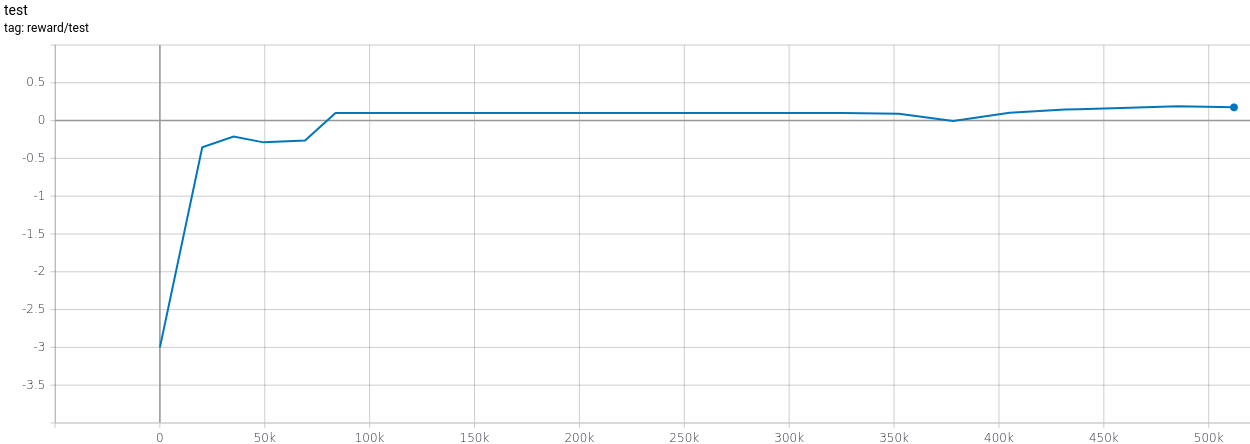
\includegraphics{figures/rl2-test-return}

Test reward is 0.1.

\subsubsection*{b) Examine the videos saved under experiments/rl2/visualize/36000/. Describe the exploration and exploitation behaviors that RL 2 learns.}
RL2 learns to visit map state however fails to exploit knowledge of the bus directions.

\subsubsection*{c) Does RL 2 achieve the optimal returns? Based on what you know about end-to-end meta-RL, do these results align with your expectations? Why or why not?}
Returns are not optimal.
This is expected because end-to-end mata-rl is difficult.

\newpage
\section*{Problem 2: Decoupled Meta-Reinforcement Learning}

\subsubsection*{a) In the grid world, the prior p(µ) is uniform over the 24 tasks. After observing a single exploration episode τ , what is the new posterior over tasks p(µ | τ )? Hint: think about what the policy does.}

If exploration policy goes to map state, posterior becomes exact.
If exploration policy gets on a bus then posterior is uniform over 6 tasks.
If exploration policy does not do any of these posterior is still uniform over 24 tasks.

\subsubsection*{b) What is the expected returns achieved by Pearl given a single exploration episode? Hint: there are two cases to consider. Show your work.}

Assuming agent gets on a bus asap.

If posterior is exact then return is $ -0.3 + 1 = 0.7 $

If posterior is uniform over 6 tasks then there are two cases to consider.
Known bus direction may be actual goal with $ 1/4 $ probability.
Known bus direction may not be actual goal with $ 3/4 $ probability in which case correct bus will be taken with a $ 1/3 $ probability.

Reaching goal will yield $0.7$ return while not reaching will yield $-0.6$ return.
$E(r) = 1/4 * 0.7 + 3/4 * (1/3* 0.7 + 2/3 * (-0.6)) =  1/4 * 0.7 + 3/4 * (-0,17) =  -0.35 $

\subsubsection*{c) Does this idealized version of Pearl achieve the optimal returns? Based on what you know about decoupled meta-RL algorithms, do these results align with your expectations? Why or why not?}

Return is not optimal. Posterior sampling is known to not look for instructions e.g. map state. This is expected.

\newpage
\section*{Problem 3: Dream}

\subsubsection*{c) Submit the plot for test returns under the tag rewards/test from the experiments/dream directory.}

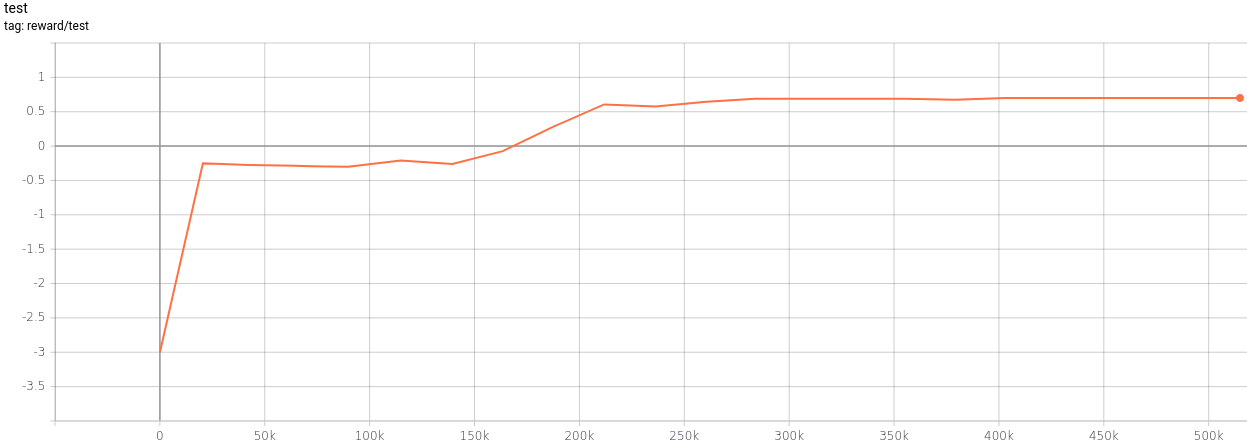
\includegraphics{figures/dream-test-return}

\subsubsection*{d) Does Dream achieve optimal returns in your results from c)? Based on what you know about Dream, do these results align with your expectations? Why or why not?}
Dream achieves test return of 0.7 which is the optimal value. This is expected.

\subsubsection*{e) Inspect the videos saved under experiments/dream/visualize/28000 or a later step after Dream converges. Describe the exploration and exploitation behaviors that Dream has learned.}
As expected dream learns to visit map state during exploration. Then in exploitation phase, correct bus is taken to target.

\end{document}

